\documentclass{beamer}
\usepackage{graphicx}
\usepackage{amsmath,amssymb,amstext,amsthm,xargs}
\usepackage{amsfonts}
\usepackage{bbm}
\usepackage{beamerthemesplit}

\usepackage[utf8]{inputenc}
\usepackage[french]{babel}
\usepackage{bbm}

\usetheme{Antibes}
\mode<presentation>
\useoutertheme{tree}
\usecolortheme{beaver}
\useinnertheme{rectangles}

\setbeamerfont{block title}{size={}}
%\usecolortheme[rgb={0.55,0.1,0.05}]{structure}
%\usecolortheme[rgb={0.75,0.1,0.05}]{structure}
\usepackage{color}

\newenvironment{disarray}{\everymath{\displaystyle\everymath{}}\array} {\endarray}
\newtheorem{theo}{Théorème}
\newtheorem{prop}[theo]{Proposition}
\newtheorem{conj}[theo]{Conjecture}
\newtheorem{cor}{Corollary}[theo]

\newtheorem{lem}{Lemme}
\newtheorem{nota}{Notation}
\newtheorem{rk}{Remark}
\newtheorem{exa}{Example}
\newtheorem{df}{Definition}
\newtheorem{terminologie}{Terminologie}
\def\rme{\mathrm{e}}
\def\rmi{\mathrm{i}}
\def\rset{\mathbb{R}}
\def\nset{\mathbb{N}}
\def\dlim{\stackrel{d}{\rightarrow}}
\newcommandx{\plim}[1][1=]{\stackrel{\PP_{#1}}{\longrightarrow}}
\def\iid{i.i.d.}
\def\1{\mathbbm{1}}
\newenvironment{dem}{\textbf{Proof}}{\flushright$\blacksquare$\\}
%\def\blankframe{
%\mode<presentation>{
%  { \setbeamertemplate{background canvas}[default]
%    \setbeamercolor{background canvas}{bg=black}
%    \begin{frame}[plain]{}
%    \end{frame}
%  }
%}
%\mode<presentation>{
%\setbeamertemplate{background canvas}[default]
%\setbeamercolor{background canvas}{bg=white}}
%\mode*
%}
\def\eqsp{\,}
\DeclareMathOperator{\E}{{\mathbb E}}
\def\PE{\E}
\def\PCov{\mathrm{Cov}}
\DeclareMathOperator{\F}{{\mathbb F}}
\DeclareMathOperator{\G}{{\mathbb G}}
\DeclareMathOperator{\D}{{\mathbb D}}
\DeclareMathOperator{\R}{{\mathbb R}}
\DeclareMathOperator{\C}{{\mathbb C}}
\DeclareMathOperator{\Z}{{\mathbb Z}}
\DeclareMathOperator{\N}{{\mathbb N}}
\DeclareMathOperator{\K}{{\mathbb K}}
\DeclareMathOperator{\T}{{\mathbb T}}
\DeclareMathOperator{\PP}{{\mathbb P}}
\DeclareMathOperator{\QQ}{{\mathbb Q}}
\DeclareMathOperator{\Q}{{\mathbb Q}}
\DeclareMathOperator{\IF}{{\mathbb I}}


%%%%%%%%%%%%%%%%%%%%%%%%%%%%%%% Pour le modèle lin\'eaire

\DeclareMathOperator{\bX}{\boldsymbol{X}}
\DeclareMathOperator{\bY}{\boldsymbol{Y}}
\DeclareMathOperator{\bx}{\boldsymbol{x}}
\DeclareMathOperator{\vp}{\boldsymbol{p}}
\DeclareMathOperator{\vq}{\boldsymbol{q}}
\DeclareMathOperator{\estMCNL}{\widehat \theta_n^{\,\,{\tt mcnl}}}
\DeclareMathOperator{\estMV}{\widehat \theta_n^{\,\,{\tt mv}}}
\DeclareMathOperator{\est}{\widehat \theta_{\mathnormal{n}}}
\DeclareMathOperator{\var}{\mathrm{Var}}
\def\Var{\var}
\DeclareMathOperator{\estMVc}{\widehat \theta_{n,0}^{\,{\tt mv}}}
\DeclareMathOperator{\Xbar}{\overline{\mathnormal{X}}_\mathnormal{n}}

\newcommand{\indi}[1]{\mathbbm{1}_{\{#1\}}}
\newcommand{\coint}[1]{\left[#1\right)}
\newcommand{\ocint}[1]{\left(#1\right]}
\newcommand{\ooint}[1]{\left(#1\right)}
\newcommand{\ccint}[1]{\left[#1\right]}

\definecolor{LightYell}{rgb}{0.95,0.83,0.70}
\definecolor{orange}{rgb}{1.0,0.50,0.01}
\definecolor{StroYell}{rgb}{0.95,0.88,0.72}
\definecolor{lightred}{rgb}{0.75,0.033,0}
\definecolor{shadecolor1}{rgb}{0.90,0.83,0.70}
\definecolor{myem}{rgb}{0.797,0.598,0.598}
\definecolor{BrickRed}{cmyk}{0,0.89,0.94,0.28}
\definecolor{RoyalPurple}{cmyk}{0.75,0.9,0,0}

\newcommand{\tco}[1]{\textcolor{orange}{#1}}
\newcommand{\tcr}[1]{\textcolor{lightred}{#1}}

\def\gauss{\mathcal{N}}
\def\truetheta{\theta}
\def\truebeta{\boldsymbol{\beta}}
\def\projX{A}
\def\curtheta{\alpha}
\def\argmin{\mathrm{argmin}}
\def\ie{\emph{i.e.}}
\def\regressmat{\mathbb{X}}
\def\errpred{\boldsymbol{\hat{\xi}}}
\def\bnoise{\boldsymbol{\xi}}
\def\predY{\hat{\mathbf{Y}}}
\DeclareMathOperator{\estregress}{\widehat{\truebeta}_n}
\DeclareMathOperator{\estMC}{\widehat \theta_n^{\,\,{\tt mc}}}
\def\curbeta{b}
\def\bcurbeta{\mathbf{b}}
\newcommand{\indep}{\rotatebox[origin=c]{90}{$\models$}} 
\newcommand{\Id}[1]{\mathrm{Id}_{#1}}

\documentclass{beamer}
\usetheme[right,hideothersubsections]{Berkeley}
\usepackage{graphicx}
\usepackage{amsmath,amssymb,amstext}
\usepackage{amsfonts}

%\usepackage[latin1]{inputenc}
\usepackage[french]{babel}
\usepackage[utf8]{inputenc}


\newenvironment{disarray}{\everymath{\displaystyle\everymath{}}\array} {\endarray}
\newtheorem{theo}{Théorme}
\newtheorem{prop}[theo]{Proposition}
\newtheorem{conj}[theo]{Conjecture}
\newtheorem{cor}{Corollary}[theo]
\newtheorem{lm}{Lemma}
\newtheorem{lemme}{Lemme}
\newtheorem{nota}{Notation}
\newtheorem{rk}{Remark}
\newtheorem{remarque}{Remarque}
\newtheorem{exa}{Example}
\newtheorem{df}{Définition}
\newtheorem{hypothese}{Hypothse}
\newtheorem{terminologie}{Terminologie}
\newenvironment{dem}{\textbf{Proof}}{\flushright$\blacksquare$\\}

\DeclareMathOperator{\E}{{\mathbb E}}
\DeclareMathOperator{\F}{{\mathbb F}}
\DeclareMathOperator{\G}{{\mathbb G}}
\DeclareMathOperator{\D}{{\mathbb D}}
\DeclareMathOperator{\R}{{\mathbb R}}
\DeclareMathOperator{\C}{{\mathbb C}}
\DeclareMathOperator{\Z}{{\mathbb Z}}
\DeclareMathOperator{\N}{{\mathbb N}}
\DeclareMathOperator{\K}{{\mathbb K}}
\DeclareMathOperator{\T}{{\mathbb T}}
\DeclareMathOperator{\PP}{{\mathbb P}}
\DeclareMathOperator{\QQ}{{\mathbb Q}}
\DeclareMathOperator{\Q}{{\mathbb Q}}
\DeclareMathOperator{\IF}{{\mathbb I}}


%%%%%%%%%%%%%%%%%%%%%%%%%%%%%%% Pour le modèle linéaire

\DeclareMathOperator{\bX}{\boldsymbol{X}}
\DeclareMathOperator{\bY}{\boldsymbol{Y}}
\DeclareMathOperator{\bx}{\boldsymbol{x}}
\DeclareMathOperator{\vp}{\boldsymbol{p}}
\DeclareMathOperator{\vq}{\boldsymbol{q}}
\DeclareMathOperator{\estMC}{\widehat \vartheta_n^{\,\,{\tt mc}}}
\DeclareMathOperator{\estMCNL}{\widehat \vartheta_n^{\,\,{\tt mcnl}}}
\DeclareMathOperator{\estMV}{\widehat \vartheta_n^{\,\,{\tt mv}}}
\DeclareMathOperator{\design}{\mathbb{M}}
\DeclareMathOperator{\est}{\widehat \vartheta_{\mathnormal{n}}}
\DeclareMathOperator{\var}{\mathrm{Var}}
\DeclareMathOperator{\estMVc}{\widehat \vartheta_{n,0}^{\,{\tt mv}}}
\DeclareMathOperator{\Xbar}{\overline{\mathnormal{X}}_\mathnormal{n}}




\title{MAP 433 : Introduction aux méthodes statistiques. Cours 6}
%\author{M. Hoffmann}
%\institute{Université Paris-Est and ETG}
\begin{document}
\date{21 mars 2014}
\maketitle



\begin{frame}
\frametitle{Aujourd'hui}
\tableofcontents
\end{frame}




%\subsection{Régression linéaire multiple}

\begin{frame}
\frametitle{Régression linéaire multiple (= Modèle linéaire)}
\begin{itemize}
\item La fonction de régression est $r(\vartheta,\bx_i) = \vartheta^T\bx_i$.
On observe
$$(\bx_1,Y_1),\ldots, (\bx_n,Y_n)$$
avec
$$\boxed{Y_i = \vartheta^T\bx_i+\xi_i,\;\;i=1,\ldots, n}$$
o $\vartheta \in \Theta = \R^k,\;\;\bx_i \in \R^k$.
\item \alert{Matriciellement}
$$\boxed{\boldsymbol{Y} = \mathbb{M}\vartheta + \boldsymbol{\xi}}$$
avec $\boldsymbol{Y} = (Y_1 \cdots Y_n)^T$, $\boldsymbol{\xi} =
(\xi_1 \cdots \xi_n)^T$ et $\mathbb{M}$ la matrice $(n\times k)$
dont les \alert{ lignes} sont les $\bx_i$.
\end{itemize}
\end{frame}

%\begin{frame}
%\frametitle{Réduction \og design\fg{} aléatoire $\longrightarrow$ déterministe}
%\begin{itemize}
%\item Les modèles de régression à \og design\fg{} déterministe ou aléatoire se traitent  \alert{ essentiellement de la mme manire} :
%\end{itemize}
%\begin{hypothese}[Ancillarité des covariables]
%On suppose que la loi $\PP^{\bX}$ des $\bX_i$ ne dépend pas du paramtre inconnu $\alert{\vartheta}$.
%\end{hypothese}
%\begin{itemize}
%\item Sous l'hypothse d'ancillarité, le caractre aléatoire des $\bX_i$ -- observés -- ne joue aucun r™le : on peut faire l'étude mathématique du modèle \alert{conditionnellement aux $\bX_i$}.
%\item \alert{ Désormais} : on se place  dans le modèle de régression à \og design \fg{} \alert{déterministe}.
%\end{itemize}
%\end{frame}
%
%\begin{frame}
%\frametitle{\og design\fg{} aléatoire vs. déterministe}
%\begin{remarque}
%{\it A posteriori} pourquoi considérer le modèle de régression à \og design \fg{} aléatoire et ne pas se placer d'emblée en signal + bruit ?
%\begin{itemize}
%\item \alert{Le design aléatoire} fournit une interprétation en terme de fonction de régression obtenue via l'espérance conditionnelle.
%\item \alert{Essentiel} pour le traitement des \alert{modèles à réponse binaire} (ou multiple), voir plus loin.
%\end{itemize}
%\end{remarque}
%\end{frame}





%\begin{frame}
%\frametitle{Estimation de $\sigma^2$}
%\begin{itemize}
%\item \alert{Estimation de $\sigma$} (ou $\sigma^2$) à partir des observations
%$$\boxed{Y_i = \vartheta_0\,+\vartheta_1\,x_i+\alert{\sigma}\, \varepsilon_i,\;\;i=1,\ldots,n}$$
%\alert{avec}
%$$\boxed{\E_\vartheta\big[\varepsilon_i\big]=0,\;\E_\vartheta\big[\varepsilon_i^2\big]=1}$$
%\item \underline{Estimateur naturel} de $\sigma^2$ :
%$$\widehat \sigma_n^2 = \frac{1}{n}\sum_{i = 1}^n\big(Y_i-r(\estMC, x_i)\big)^2$$
%\item Somme de variables aléatoires \alert{non indépendantes}.
%\item Difficile de progresser \alert{sans hypothse supplémentaire}. Si les $\varepsilon_i$ sont i.i.d. ${\mathcal N}(0,1)$, alors \alert{on sait} \og résoudre \fg{} le problme... plus loin.
%\end{itemize}
%\end{frame}





%\subsection{EMV et EMC}

\begin{frame}
\frametitle{EMC en régression linéaire multiple}
\begin{itemize}
\item Estimateur des \alert{moindres carrés} en régression
linéaire multiple : tout estimateur $\estMC$ satisfaisant
$$\sum_{i = 1}^n
\big(Y_i-(\estMC)^T\bx_i\big)^2 = \min_{\vartheta \in \R^k}\sum_{i =
1}^n \big(Y_i-{\vartheta}^T\bx_i\big)^2.$$
\item En notation matricielle :
\begin{eqnarray*} \|\boldsymbol{Y}-\design\estMC\|^2 &=& \min_{\vartheta \in
\R^k}\|\boldsymbol{Y}-\design\vartheta\|^2\\
&=& \min_{v \in V}\|\boldsymbol{Y}-v\|^2
\end{eqnarray*}
o\`u $V=\text{Im}(\design) = \{v\in \R^n: v=\design\vartheta, \
\vartheta\in \R^k\}$.
 Projection orthogonale sur $V$.
 \end{itemize}
 \end{frame}

% \subsection{Géometrie de l'EMC}

 \begin{frame}
\frametitle{Géométrie de l'EMC}
 \begin{itemize}
 \item L'EMC vérifie
$$\boxed{\design {\estMC} = P_V \boldsymbol{Y}}$$
o\`u $P_V$ est le projecteur orthogonal sur $V$.
\item Mais $\design^T  P_V= \design^T  P_V^T = ( P_V\design)^T =
\design^T$. On en déduit \alert{les équations normales des
moindres carrés}:
$$\boxed{\design^T\design {\estMC} =
\design^T\boldsymbol{Y}.}$$
\item \underline{Remarques.}
  \begin{itemize}
  \item L'EMC est un $Z$-estimateur.
  \item Pas d'\alert{unicité} de $\estMC$ si la matrice
  $\design^T\design$ n'est pas inversible.
  \end{itemize}
\end{itemize}
\end{frame}

\begin{frame} \frametitle{Géométrie de l'EMC}
\begin{prop}
Si $\design^T\design$ (matrice $k \times k$) inversible, alors
$\estMC$ \alert{est unique} et
$$\boxed{\estMC = \big(\design^T\design\big)^{-1}\design^T \boldsymbol{Y}}$$
\end{prop}
\begin{itemize}
\item Contient  la droite de régression simple.
\item Résultat géometrique, \alert{non stochastique}.
%\item $\design^T\design\ge0$; \ \ $\design^T\design$
%inversible $\Longleftrightarrow$ $\design^T\design>0$;
%$$\design^T\design>0 \ \Longleftrightarrow \ {\rm rang}(\design)=k
%\ \Longleftrightarrow \ {\rm dim}(V)=k.$$
%$$\design^T\design>0 \quad \Longrightarrow \quad \alert{ n \geq k}.$$
\end{itemize}
\end{frame}














%\subsection{Le cas gaussien}





%\section{Régression linéaire : rappels}
%
%\subsection{Régression à \og design \fg{} déterministe}
%
%\begin{frame}
%\frametitle{Modèle de régression}
%\begin{df}
%Modèle de régression (à \og design\fg{} déterministe) = donnée de l'observation
%$$(\bx_1,Y_1),\ldots, (\bx_n,Y_n)$$
%avec $Y_i \in \R, \bx_i\in \R^k$, et
%$$Y_i = r(\alert{\vartheta},\bx_i)+\xi_i,\;\;\E\big[\xi_i\big]=0,\;\;\alert{ \vartheta \in \Theta \subset \R^d}.$$
%\begin{itemize}
%%\item $\bx \leadsto r(\alert{\vartheta},\bx)$ fonction de \alert{ régression}, connue au paramtre
%%$\vartheta$ prs.
%\item $\bx_i$ déterministes, donnés (ou choisis) : plan d'expérience, points du \og design\fg{}.
%\item Hypothse : les $\xi_i$ sont i.i.d. (pour simplifier). \alert{ Attention : } les $Y_i$ ne sont \alert{pas} identiquement distribuées.
%\item Ecriture de la vraisemblance du modèle...
%\end{itemize}
%\end{df}
%\end{frame}
%
%
%\begin{frame}
%\frametitle{Modèle linéaire}
%\begin{itemize}
%\item On observe
%$$(\bx_1,Y_1),\ldots, (\bx_n,Y_n)$$
%avec
%$$\boxed{Y_i = \vartheta^T\bx_i+\xi_i,\;\;i=1,\ldots, n}$$
%o $\vartheta \in \Theta = \R^k,\;\;\bx_i \in \R^k$.
%\item \alert{Matriciellement}
%$$\boxed{\boldsymbol{Y} = \mathbb{M}\vartheta + \boldsymbol{\xi}}$$
%avec $\boldsymbol{Y} = (Y_1,\ldots, Y_n)^T$, $\boldsymbol{\xi} = (\xi_1,\ldots, \xi_n)^T$ et $\mathbb{M}$ la matrice $(n\times k)$ dont les \alert{ lignes} sont les $\bx_i$.
%\end{itemize}
%\end{frame}
%
%%%\subsection{EMV et EMC}
%
%\begin{frame}
%\frametitle{Estimateur des moindres carrés}
%\begin{df}
%\alert{Estimateur des moindres carrés} (EMC) : tout estimateur
%$\estMC$ satisfaisant $\estMC \in \arg \min_{\vartheta \in
%\R^k}\sum_{i = 1}^n \big(Y_i-\vartheta^T\bx_i\big)^2$.
%\end{df}
%
%\begin{itemize}
%\item
%EMC = cas particulier de $M$-estimateur et de $Z$-estimateur
%\end{itemize}
%
%\begin{prop}
%Si $\design^T\design$ (matrice $k \times k$) inversible (cond. néc. : $\alert{ n \geq k}$), alors $\estMC$ \alert{est unique} et
%$$\boxed{\estMC = \big(\design^T\design\big)^{-1}\design^T \boldsymbol{Y}}$$
%\end{prop}
%\end{frame}
%



%\subsection{Modèle linéaire gaussien}


%\subsection{Propriétés statistiques de l'EMC : cas gaussien}

\begin{frame}
\frametitle{Cadre gaussien : loi des estimateurs}
\begin{itemize}
\item \underline{Hyp. 1} : $\boldsymbol{\xi} \sim {\mathcal N}(0,\sigma^2\mathrm{Id}_n)$.
\item \underline{Hyp. 2} : $\design^T \design>0$.
\end{itemize}
\begin{prop}
\begin{itemize}
\item[(i)] $\estMC \sim {\mathcal N}\big(\vartheta, \sigma^2 \big(\design^T\design\big)^{-1}\big)$
\item[(ii)] $\|\boldsymbol{Y}-\design \estMC\|^2 \sim
\sigma^2\chi^2(n-k)$ \alert{ loi du Chi 2 à $n-k$ degrés de liberté}
\item[(iii)] $\estMC$ et $\boldsymbol{Y}-\design \estMC$ sont indépendants.
\end{itemize}
\end{prop}
\begin{itemize}
\item \underline{Preuve} : \alert{Thm. de Cochran} (Poly, page 18). Si
$\boldsymbol{\xi}\sim {\mathcal N}(0,\mathrm{Id}_n)$ et $A_j$
matrices $n \times n$ projecteurs t.q. $A_jA_i=0$ pour $i\neq j$,
alors : $A_j\,\boldsymbol{\xi} \sim {\mathcal N}\big(0,A_j\big)$,
\alert{indépendants}, $\|A_j\boldsymbol{\xi}\|^2\sim
\chi^2(\mathrm{Rang}(A_j))$.
\end{itemize}
\end{frame}



\begin{frame}
\frametitle{Propriétés de l'EMC: cadre gaussien}

Estimateur de la variance $\sigma^2$:
$$\boxed{\widehat \sigma_n^2 = \frac{\|\boldsymbol{Y}-\design \estMC\|^2}{n-\alert{k}} = \frac{1}{n-\alert{k}}\sum_{i = 1}^n\big(Y_i-(\estMC)^T\bx_i\big)^2}$$
D'apr\`es la derni\`ere Proposition :
\begin{itemize}
\item $\widehat
\sigma_n^2/\sigma^2 \sim \chi^2(n-k)$ \alert{ loi du Chi 2 à
$n-k$ degrés de liberté}
\item C'est un estimateur \alert{sans biais}: $$\E_\vartheta\big[\widehat
\sigma_n^2\big]=\sigma^2.$$
\item $\widehat
\sigma_n^2$ est \alert{indépendant} de $\estMC$.
\end{itemize}
\end{frame}

\begin{frame}
\frametitle{Propriétés de l'EMC: cadre gaussien}
\begin{itemize}
\item Lois des coordonnées de $\estMC$:
$$
(\estMC)_j -\vartheta_j \sim {\mathcal N}\big(0, \sigma^2 b_j)
$$
o\`u $b_j$ est le $j$\`eme élément diagonal de $\big(\design^T
\design\big)^{-1}$. $$ \frac{(\estMC)_j -\vartheta_j}{\widehat
\sigma_n \sqrt{b_j}} \sim t_{n-k}$$ \alert{loi de Student \`a
$n-k$ degrés de liberté}.
$$ t_q = \frac{\xi}{\sqrt{\eta/q}}$$
o\`u $q\ge 1$ un entier, $\xi\sim {\mathcal N}\big(0,1)$, $\eta\sim
\chi^2(q)$ et\\ $\xi$ \alert{indépendant} de $\eta$.
\end{itemize}
\end{frame}

\begin{frame}
    \frametitle{Exemple de données de régression}
\begin{center}
\vspace{-2.5cm}
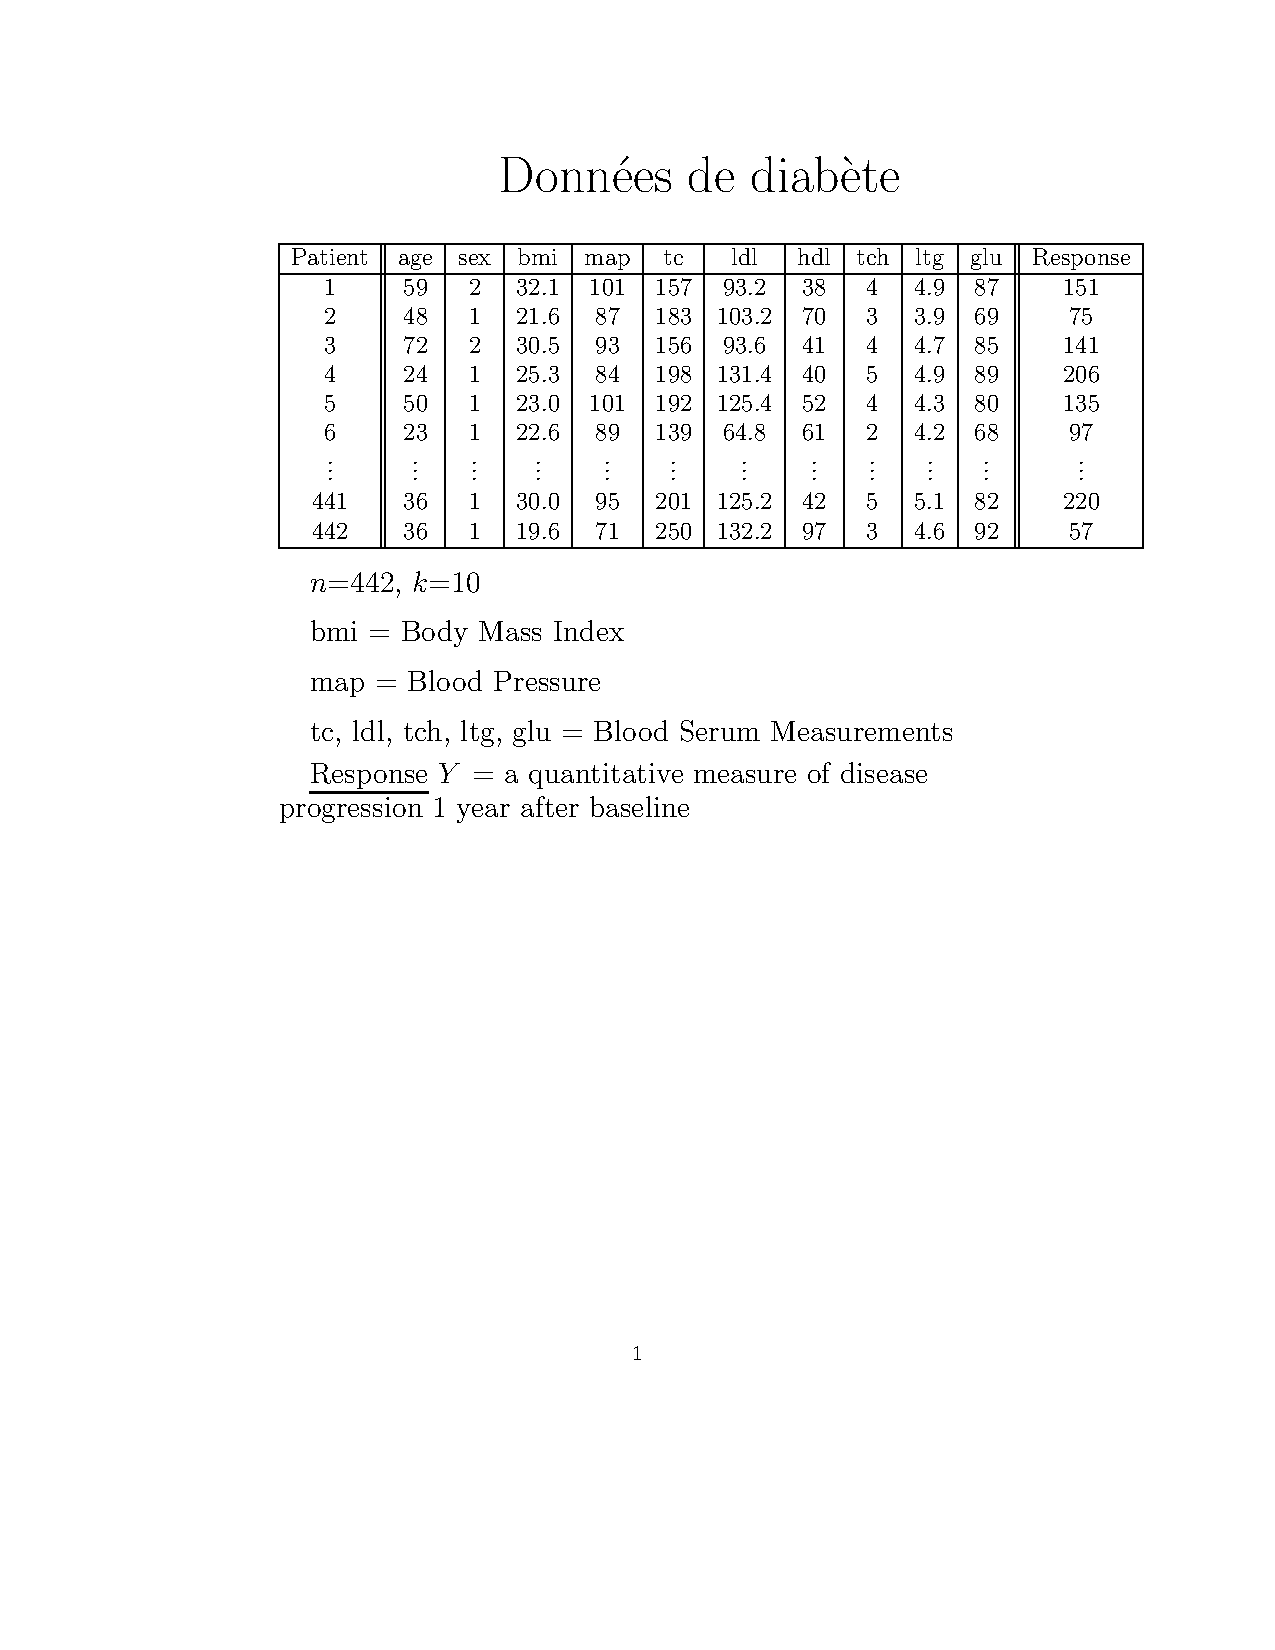
\includegraphics[height=2\textheight]{cours4_data1.pdf}\hspace{4cm}
\end{center}
\end{frame}

\begin{frame}
\frametitle{Résultats de traitement statistique initial}
\begin{tabular}{|c||c|c|c|c|}
\hline &Estimate&Std. Error&t value&Pr($>|t|$)\\\hline
(Intercept) &$152.133$&$2.576$&$59.061$&$< 2e-16***$\\
age&$-10.012$&$59.749$&$ -0.168$&$0.867000$\\\hline
sex &$-239.819$&$61.222$&$-3.917$&$0.000104***$\\
bmi&$519.840$&$66.534$&$7.813$&$4.30e-14***$\\\hline
map&$324.390$&$65.422$&$4.958$&$1.02e-06***$\\
tc&$-792.184$&$416.684$&$-1.901$&$0.057947$\\\hline
ldl&$476.746$&$339.035$&$1.406$&$0.160389$\\
hdl&$101.045$&$212.533 $&$0.475$&$0.634721$\\\hline
tch&$177.064$&$161.476$&$ 1.097$&$0.273456$\\
ltg&$751.279$&$ 171.902$&$4.370$&$ 1.56e-05***$\\\hline
glu&$67.625$&$ 65.984$&$1.025$&$0.305998$\\\hline
\end{tabular}
\end{frame}

\begin{frame}
\frametitle{Questions statistiques}
\begin{itemize}
\item {\bf Sélection de variables.} Lesquelles parmi les 10
variables:\\\vspace{3mm}
\centerline{\texttt{age,sex,bmi,map,tc,ldl,hdl,tch,ltg,glu}}\vspace{3mm}
sont significatives? Formalisation mathématique: trouver (estimer)
l'ensemble $N= \{j: \vartheta_{j}\ne 0\}$.
\item {\bf Prévison.} Un nouveau patient arrive avec son vecteur
des 10 variables ${\bf x}_0\in \R^{10}$. Donner la prévison de la
réponse $Y$ =état du patient dans 1 an.
\end{itemize}
\end{frame}

\section{Sélection de variables}

\begin{frame}
\frametitle{RSS (Residual Sum of Squares)} Mod\`ele de
régression\vspace{2mm} \centerline{$ Y_i= r(\vartheta, {\bf
x}_i)+\xi_i, \quad i=1,\dots,n.$}
\begin{itemize}
\item {\bf Résidu:} si $\est$ est un estimateur de
$\vartheta$,
$$\widehat \xi_i = Y_i - r(\est, {\bf x}_i)
\;\;\text{\alert{résidu} au point}\;i.$$
\item {\bf RSS:} \alert{ Residual Sum of Squares}, somme
résiduelle des carrés. Caractérise la qualité
d'approximation.
$${\rm RSS}(={\rm RSS}_{\est})=\|\widehat \xi\|^2
= \sum_{i = 1}^n\big(Y_i - r(\est,{\bf x}_i)\big)^2.$$
\item En régression \alert{linéaire}:
$\boxed{{\rm RSS}= \|{\bf Y}-\design\est\|^2.}$
\end{itemize}
\end{frame}

\subsection{Backward Stepwise Regression}

\begin{frame}
\frametitle{Sélection de variables : Backward Stepwise Regression}
\begin{itemize}
\item On se donne un crit\`ere d'élimination de variables
\alert{(plusieurs choix de crit\`ere possibles...)}.
\item On élimine une
variable, la moins significative du point de vue du crit\`ere
choisi.
\item On calcule l'EMC $\widehat\vartheta_{n,k-1}^{\rm mc}$ dans le nouveau mod\`ele, avec seulement
les $k-1$ paramétres restants, ainsi que le RSS:\vspace{1mm}
\centerline{${\rm RSS}_{k-1}=\|{\bf
Y}-\design\widehat\vartheta_{n,k-1}^{\rm mc}\|^2$.}\vspace{1mm}
\item On continue \`a éliminer des variables, une par une,
jusqu'\`a la \alert{stabilisation de RSS}: ${\rm
RSS}_{m}\approx {\rm RSS}_{m-1}$.
\end{itemize}
\end{frame}


\begin{frame}
\frametitle{Données de diab\`ete : Backward Regression}

\begin{itemize}
\item {\bf Sélection "na\"{\i}ve"} : \
\{\texttt{sex,bmi,map,ltg}\}
\item {\bf Sélection par Backward Regression}:\\
 \alert{Crit\`ere
d'élimination: plus grande valeur de} Pr($>|t|$).
\end{itemize}
%\vspace{2mm}


{\small
\begin{tabular}{|c||c|c|c|c|}
\hline &Estimate&Std. Error&t value&Pr($>|t|$)\\\hline
(Intercept) &$152.133$&$2.576$&$59.061$&$< 2e-16***$\\
\alert{age}&$-10.012$&$59.749$&$
-0.168$&$\alert{0.867000}$\\\hline
sex &$-239.819$&$61.222$&$-3.917$&$0.000104***$\\
bmi&$519.840$&$66.534$&$7.813$&$4.30e-14***$\\\hline
map&$324.390$&$65.422$&$4.958$&$1.02e-06***$\\
tc&$-792.184$&$416.684$&$-1.901$&$0.057947$\\\hline
ldl&$476.746$&$339.035$&$1.406$&$0.160389$\\
hdl&$101.045$&$212.533 $&$0.475$&$0.634721$\\\hline
tch&$177.064$&$161.476$&$ 1.097$&$0.273456$\\
ltg&$751.279$&$ 171.902$&$4.370$&$ 1.56e-05***$\\\hline
glu&$67.625$&$ 65.984$&$1.025$&$0.305998$\\\hline
\end{tabular}
}
\end{frame}

\begin{frame}
\frametitle{Données de diab\`ete : Backward Regression}

\centerline{\bf Backward Regression: Itération 2.}

%\vspace{3mm}

\begin{center}

\alert{Crit\`ere d'élimination: plus grande valeur de}
Pr($>|t|$).

\vspace{4mm}

{\small
\begin{tabular}{|c||c|c|c|c|}
\hline &Estimate&Std. Error&t value&Pr($>|t|$)\\\hline (Intercept)
&$152.133$&$2.573$&$59.128$&$< 2e-16$
\\\hline
sex &$-240.835$&$60.853$&$-3.958$&$0.000104$\\
bmi&$519.905$&$64.156$&$5.024$&$8.85e-05$\\\hline
map&$322.306$&$65.422$&$4.958$&$7.43e-07$\\
tc&$-790.896$&$416.144$&$-1.901$&$0.058$\\\hline
ldl&$474.377$&$338.358$&$1.402$&$0.162$\\
\alert{ hdl}&$99.718$&$212.146 $&$0.470$&$\alert{
0.639}$\\\hline
tch&$177.458$&$161.277$&$ 1.100$&$0.272$\\
ltg&$749.506$&$ 171.383$&$4.373$&$ 1.54e-05$\\\hline glu&$67.170$&$
65.336$&$1.013$&$0.312$\\\hline
\end{tabular}
}
\end{center}
\end{frame}

\begin{frame}
\frametitle{Données de diab\`ete : Backward Regression}

\centerline{\bf Backward Regression: Itération 5 (derni\`ere).}

%\vspace{3mm}

\begin{center}

Variables sélectionnées:\\\vspace{2mm}
\{\texttt{sex,bmi,map,\alert{tc,ldl},ltg}\}


\vspace{4mm}

{\small
\begin{tabular}{|c||c|c|c|c|}
\hline &Estimate&Std. Error&t value&Pr($>|t|$)\\\hline (Intercept)
&$152.133$&$2.572$&$59.159$&$< 2e-16$
\\\hline
sex &$-226.511$&$59.857$&$-3.784$&$0.000176$\\
bmi&$529.873$&$65.620$&$8.075$&$6.69e-15$\\\hline
map&$327.220$&$62.693$&$5.219$&$2.79e-07$\\
tc&$-757.938$&$160.435$&$-4.724$&$3.12e-06$\\\hline
ldl&$538.586$&$146.738$&$3.670$&$0.000272$\\
ltg&$804.192$&$80.173$&$10.031$&$< 2e-16$\\\hline
\end{tabular}
}
\end{center}
\end{frame}

\begin{frame}
\frametitle{Sélection de variables : Backward Regression}

Discussion de \texttt{Backward Regression}:

\begin{itemize}
\item Méthode de sélection purement empirique, pas de justification
théorique.
\item Application d'autres crit\`eres d'élimination en
\texttt{Backward Regression} peut amener aux résultats différents.\\
\underline{Exemple.} \alert{Crit\`ere $C_p$} de Mallows--Akaike
: on élimine la variable $j$ qui réalise
$$
\min_j \Big({\rm RSS}_{m, (-j)} + 2\widehat\sigma^2_n m\Big).
$$
\end{itemize}
\end{frame}

\subsection{LASSO}

\begin{frame}
\frametitle{Sélection de variables : LASSO}

LASSO = Least Absolute Shrinkage and Selection Operator

\begin{itemize}
\item \alert{Estimateur LASSO}: tout estimateur $\widehat\vartheta^{L}_n$
vérifiant
$$\widehat\vartheta^{L}_n \in \arg \min_{\vartheta \in \R^k}\left(\sum_{i = 1}^n
\big(Y_i-\vartheta^T\bx_i\big)^2 + \lambda \sum_{j =
1}^k|\vartheta_j|\right) \ \ \text{avec} \ \lambda>0.
$$
\item Si $\design^T\design>0$, l'estimateur LASSO $\widehat\vartheta^{L}_n$ est unique.
\item Estimateur des moindres carrés \alert{pénalisé}.
Pénalisation par $\sum_{j = 1}^k|\vartheta_j|$, la norme $\ell_1$
de $\vartheta$.
\end{itemize}
\end{frame}

\begin{frame}
\frametitle{Sélection de variables : LASSO}
\begin{itemize}
\item Deux utilisations de
LASSO:
\begin{itemize}
\item \alert{Estimation de $\vartheta$}: alternative \`a
$\estMC$ si $k>n$.
\item \alert{Sélection de variables}: on ne retient que les
variables qui correspondent aux coordonnées non-nulles du vecteur
$\widehat\vartheta^{L}_n$.
\end{itemize}
\item LASSO admet une \alert{justification théorique}: sous certaines hypoth\`eses sur la
matrice $\design$,
$$
\lim_{n\to\infty} \PP\{ \widehat N_n = N \} =1,
$$
o\`u $N= \{j: \vartheta_{j}\ne 0\}$ et $\widehat N_n= \{j:
\widehat\vartheta^{L}_{n,j}\ne 0\}$.
\end{itemize}
\end{frame}

\begin{frame}
    \frametitle{Application de LASSO: "regularization path"}
\begin{center}
\vspace{-1cm}
\includegraphics[height=1.35\textheight,angle=-90]{cours4_sacha_graphe.eps}\hspace{3cm}
\end{center}
\end{frame}

\begin{frame}
\frametitle{Données de diab\`ete : LASSO}

Application aux données de diab\`ete.

\begin{itemize}
\item  L'ensemble de variables sélectionné par LASSO:
$$
\{\texttt{sex,bmi,map,tc,hdl,ltg,glu}\}
$$
\item \texttt{Backward Regression}:
$$
\{\texttt{sex,bmi,map,tc,ldl,ltg}\}
$$
\item Sélection na\"{\i}ve:
$$
\{\texttt{sex,bmi,map,tc}\}
$$
\end{itemize}
\end{frame}


%\section{Prévision}

%\begin{frame}
%\frametitle{Prévision}
%
%Mod\`ele de régression \vspace{2mm} \centerline{$ Y_i=
%r(\vartheta, {\bf x}_i)+\xi_i, \quad i=1,\dots,n.$} Régression
%\alert{linéaire}: $r(\vartheta, {\bf x}_i)=\vartheta^T{\bf
%x}_i$. Exemple: ${\bf x}_i$ vecteur de 10 variables explicatives
%(\texttt{age,sex,bmi,...}) pour patient $i$.
%\begin{itemize}
%\item {\bf Probl\`eme de prévision}:
%Un nouveau patient arrive avec son vecteur des 10 variables ${\bf
%x}_0\in \R^{10}$. Donner la prévison de la valeur de fonction de
%régression $r(\vartheta, {\bf x}_0)=\vartheta^T{\bf x}_0$\\
%(=état du patient dans 1 an).
%\item Soit $\est$ un estimateur de $\vartheta$. \alert{Prévision par
%substitution:}
% \centerline{$\boxed{ \widehat Y = r(\est, {\bf x}_0).}$}
%\item \underline{Question statistique}: quelle est la qualité de la prévision?
%\alert{Intervalle de confiance} pour $r(\vartheta, {\bf x}_0)$
%basé sur $\widehat Y$?
%\end{itemize}
%\end{frame}
%
%\begin{frame}
%\frametitle{Prévision: mod\`ele linéaire gaussienne}
%\begin{itemize}
%\item Traitement sur l'exemple: $r(\vartheta, {\bf x})=\vartheta^T{\bf
%x}$, régression \alert{linéaire gaussienne} et
%$\est=\estMC$. $\Longrightarrow$ $\boxed{\widehat Y = {\bf
%x}_0^T\estMC}$
%\item \underline{Hyp. 1} : $\boldsymbol{\xi} \sim {\mathcal N}(0,\sigma^2\mathrm{Id}_n)$.
%\item \underline{Hyp. 2} : $\design^T \design>0$.
%\end{itemize}
%\begin{prop}
%\begin{itemize}
%\item[(i)] $\widehat Y \sim {\mathcal N}\big({\bf
%x}_0^T\vartheta, \sigma^2 {\bf
%x}_0^T\big(\design^T\design\big)^{-1}{\bf x}_0\big)$
%\item[(ii)] $\widehat Y-{\bf
%x}_0^T\vartheta$ et $\boldsymbol{Y}-\design \estMC$ sont
%indépendants.
%\end{itemize}
%\end{prop}
%Rappel: $\|\boldsymbol{Y}-\design \estMC\|^2 \sim
%\sigma^2\chi^2(n-k)$ \alert{ loi du Chi 2 à $n-k$ degrés de
%liberté}.
%\end{frame}
%
%\begin{frame}
%\frametitle{Prévision: mod\`ele linéaire gaussienne}
%\begin{itemize}
%\item D'apr\`es la Proposition,
%$$
%\eta:=\frac{\widehat Y -{\bf x}_0^T\vartheta} {\sqrt{\sigma^2 {\bf
%x}_0^T\big(\design^T\design\big)^{-1}{\bf x}_0}}\sim {\mathcal
%N}(0,1).
%$$
%\item On replace $\sigma^2$ inconnu par $\widehat \sigma_n^2 =
%{\|\boldsymbol{Y}-\design \estMC\|^2}/({n-k}).$
%\item \alert{$t$-statistique:}
%$$
%t:= \frac{\widehat Y -{\bf x}_0^T\vartheta} {\sqrt{\widehat
%\sigma_n^2 {\bf x}_0^T\big(\design^T\design\big)^{-1}{\bf
%x}_0}}=\frac{\eta}{\sqrt{\chi/(n-k)}}\sim t_{n-k},
%$$
%\alert{loi de Student à $n-k$ degrés de liberté}, car $\eta\sim
%{\mathcal N}(0,1)$, $\chi:=\|\boldsymbol{Y}-\design
%\estMC\|^2/\sigma^2\sim \chi^2(n-k)$ et $\eta\ind\chi$.
%\end{itemize}
%\end{frame}
%
%\begin{frame}
%\frametitle{Prévision: intervalle de confiance}
%\begin{eqnarray*}
%&&\PP \Big(-q_{1-\frac{\alpha}{2}}(t_{n-k}) \le \frac{\widehat Y
%-{\bf x}_0^T\vartheta} {\sqrt{\widehat \sigma_n^2 {\bf
%x}_0^T\big(\design^T\design\big)^{-1}{\bf x}_0}}\le
%q_{1-\frac{\alpha}{2}}(t_{n-k})\Big) \\\hspace{4mm} &&= \PP(-
%q_{1-\frac{\alpha}{2}}(t_{n-k}) \le t\le
%q_{1-\frac{\alpha}{2}}(t_{n-k})) = 1-\alpha.
%\end{eqnarray*}
%$\Longrightarrow$ \alert{intervalle de confiance} de niveau
%$1-\alpha$ pour $r(\vartheta,{\bf x}_0)={\bf x}_0^T\vartheta$ est
%\alert{$[r_L, r_U]$}, o\`u:
%\begin{eqnarray*}
%\alert{r_L}&=&\widehat Y -
%q_{1-\frac{\alpha}{2}}(t_{n-k})\sqrt{\widehat \sigma_n^2
%{\bf x}_0^T\big(\design^T\design\big)^{-1}{\bf x}_0},\\
%\alert{r_U}&=& \widehat Y +
%q_{1-\frac{\alpha}{2}}(t_{n-k})\sqrt{\widehat \sigma_n^2 {\bf
%x}_0^T\big(\design^T\design\big)^{-1}{\bf x}_0}.
%\end{eqnarray*}
%\end{frame}



\begin{frame}
\frametitle{Limites des moindres carrés et du cadre gaussien}
\begin{itemize}
\item Calcul \alert{explicite} (et efficace) de l'EMC  limité à
une fonction de régression \alert{linéaire}.
\item Mod\`ele linéaire donne un cadre assez général:
\begin{itemize}
\item Mod\`ele
polynomial, \item \alert{Mod\`eles avec interactions...}
\end{itemize}
\item \alert{ Hypothse de gaussianité} = cadre asymptotique implicite.
\item Besoin d'outils pour les modèles  à réponse \alert{$Y$ discrte}.
\end{itemize}
\end{frame}

%\section{Régression linéaire non-gaussienne}

\begin{frame}
\frametitle{Régression linéaire non-gaussienne} Mod\`ele de
régression linéaire \vspace{3mm} \centerline{$ Y_i= \vartheta^T
{\bf x}_i+\xi_i, \quad i=1,\dots,n.$}

\vspace{-2mm}

\begin{itemize}
\item \underline{Hyp. 1'} : \alert{$\xi_i$ i.i.d., $\E[\xi_i]
=0$, $\E[\xi_i^2] = \sigma^2>0$.}
\item \underline{Hyp. 2'} : $\design^T \design>0$, \alert{$\lim_n\max_{1\le i \le n}{\bf x}_i^T
\big(\design^T \design\big)^{-1}{\bf x}_i =0$.}
\end{itemize}
\begin{prop}[Normalité asymptotique de l'EMC]
$$
\sigma^{-1}\big(\design^T
\design\big)^{1/2}(\estMC-\vartheta)\stackrel{d}{\longrightarrow}
{\mathcal N}\big(0, \mathrm{Id}_k), \quad n\to\infty.
$$
\end{prop}
\begin{itemize}
\item A comparer avec le cadre gaussien:\vspace{2mm}
\centerline{$\sigma^{-1}\big(\design^T
\design\big)^{1/2}(\estMC-\vartheta)\sim {\mathcal N}\big(0,
\mathrm{Id}_k)$ \text{pour tout $n$.}}
\end{itemize}
\end{frame}

%\begin{frame}
%\frametitle{Vitesses de convergence}
%\end{frame}

%\subsection{Propriété de l'EMC: cadre général (non-gaussien) }
%
%\begin{frame}
%\begin{itemize}
%\item \underline{Hyp. 1} : $\design^T \design$ inversible
%\item  \underline{Hyp. 2} :
%\alert{$\E\big[\boldsymbol{\xi}\big]=0$,
%$\E\big[\boldsymbol{\xi}\boldsymbol{\xi}^T\big] = \sigma^2
%\mathrm{Id}_n$}.
%\end{itemize}
%\begin{prop}
%%Sous les hypothses précédentes
%\begin{itemize}
%\item $\E_\vartheta\big[\estMC\big]=\vartheta$ et
%$$\E_\vartheta\big[\big(\estMC-\vartheta\big)\big(\estMC-\vartheta\big)^T\big]=\sigma^2 \big(\design^T\design\big)^{-1}$$
%\item Si l'on pose
%$$\boxed{\widehat \sigma_n^2 = \frac{\|\boldsymbol{Y}-\design \estMC\|^2}{n-\alert{k}} = \frac{1}{n-\alert{k}}\sum_{i = 1}^n\big(Y_i-(\estMC)^T\bx_i\big)^2}$$
%alors $\E_\vartheta\big[\widehat \sigma_n^2\big]=\sigma^2.$
%\end{itemize}
%\end{prop}
%\end{frame}





\section{Régression non-linéaire}


\begin{frame}
\frametitle{Régression non-linéaire}
\begin{itemize}
\item On observe
$$(\bx_1,Y_1),\ldots, (\bx_n,Y_n),$$
o
$$\boxed{Y_i = r(\alert{\vartheta},\bx_i)+\xi_i,\;\;i=1,\ldots,n}$$
avec
$$\bx_i\in \R^k,\;\;\text{et}\;\; \alert{\vartheta \in \Theta \subset \R^d}.$$
\item Si $\xi_i \sim_{\text{i.i.d.}} {\mathcal N}(0,\sigma^2)$,
$${\mathcal L}_n(\vartheta, Y_1,\ldots, Y_n) \propto \exp\Big(-\frac{1}{2\sigma^2}\sum_{i = 1}^n\big(Y_i-r(\vartheta,\bx_i)\big)^2\Big)$$
et l'estimateur du \alert{maximum de vraisemblance} est obtenu en minimisant la fonction
$$\vartheta \leadsto \sum_{i = 1}^n\big(Y_i-r(\vartheta,\bx_i)\big)^2.$$
\end{itemize}
\end{frame}

\begin{frame}
\frametitle{Moindre carrés non-linéaires}
\begin{df}
\begin{itemize}
\item $M$-estimateur associé à la \alert{fonction de contraste} $\psi:\Theta \times \alert{\R^k}\times \R\rightarrow \R$ : tout estimateur $\est$ satisfaisant
$$\sum_{i = 1}^n \psi(\est, \bx_i, Y_i) = \max_{a \in \Theta} \sum_{i = 1}^n \psi(a,\bx_i,Y_i).$$
\item Estimateur des \alert{moindres carrés non-linéaires} : associé au contraste $\psi(a,\bx,y) = -\big(y-r(a,\bx)\big)^2$.
\end{itemize}
\end{df}
\begin{itemize}
\item \alert{Extension} des résultats en densité
$\rightarrow$ théormes limites pour des sommes de v.a.
indépendantes \alert{ non-équidistribuées}.
\end{itemize}
\end{frame}

\begin{frame}
\frametitle{Modèle à réponse binaire}
\begin{itemize}
\item On observe
$$(\bx_1,Y_1),\ldots, (\bx_n,Y_n),\;\;\alert{Y_i \in \{0,1\}},\;\bx_i \in \R^k.$$
\item Modélisation \alert{via la fonction de régression}
$$\bx \leadsto p_{\bx}(\vartheta) = \E_\vartheta\big[Y|\bX = \bx\big] = \PP_\vartheta\big[Y = 1|\bX=\bx\big]$$
%$$Y_i = p_{\bx_i}(\vartheta)+\big(Y_i-p_{\bx_i}(\vartheta)\big)$$
\item \alert{Représentation}
\begin{align*}
Y_i & =  p_{\bx_i}(\vartheta)+\big(Y_i-p_{\bx_i}(\vartheta)\big) \\
& = r(\vartheta,\bx_i)+\xi_i
\end{align*}
avec
$r(\vartheta, \bx_i) = p_{\bx_i}(\vartheta)$ et $\xi_i = Y_i-p_{\bx_i}(\vartheta).$
\item $\E_\vartheta\big[\xi_i\big]=0$ mais structure des $\xi_i$ \alert{compliquée} (dépendance en $\vartheta$).
\end{itemize}
\end{frame}

\begin{frame}
\frametitle{Modèle à réponse discrte}
\begin{itemize}
\item $Y_i $ v.a. de Bernoulli de paramtre $p_{\bx_i}(\alert{\vartheta})$.

\alert{ Vraisemblance}
$${\mathcal L}_n(\vartheta,Y_1,\ldots, Y_n) = \prod_{i = 1}^n p_{\bx_i}(\alert{\vartheta})^{Y_i}(1-p_{\bx_i}\big(\alert{\vartheta})\big)^{1-Y_i}$$
$\rightarrow$ méthodes de résolution numérique.
\item \alert{ Régression logistique} (trs utile dans les applications)
$$p_{\bx}(\vartheta) = \psi(\bx^T\vartheta),$$
$$\psi(t)=\frac{e^t}{1+e^t},\;t \in \R\;\;\alert{{\text{fonction logistique}}}.$$
\end{itemize}
\end{frame}

\begin{frame}
\frametitle{Régression logistique et modèles latents}
\begin{itemize}
\item \alert{Représentation équivalente de la régression logistique} : on observe
$$\boxed{Y_i = 1_{\big\{Y_i^\star >0\big\}},\;\;i=1,\ldots,n}$$
(les $\bx_i$ sont donnés), et $Y_i^\star$ est une  \alert{variable latente} ou cachée,
$$\boxed{Y^\star_i =\alert{\vartheta}^T \bx_i + U_i,\;\;i=1,\ldots, n}$$
avec \alert{$U_i\sim_{\text{i.i.d.}} F$}, o
$$F(t) = \frac{1}{1+e^{-t}},\;t \in \R.$$
\item
\begin{align*}
\PP_\vartheta\big[Y_i^\star>0] & = \PP_\vartheta\big[\bx_i^T\vartheta + U_i >0\big] \\
& = 1-\PP_\vartheta\big[U_i \leq -\bx_i^T\vartheta\big] \\
& = 1-\big(1+\exp(-\bx_i^T\vartheta)\big)^{-1} =  \psi(\bx_i^T\vartheta).
\end{align*}
\end{itemize}
\end{frame}



\section{Comparaison d'estimateurs}

\begin{frame}
\frametitle{Bilan provisoire : modèles paramétriques dominés}
%, construction d'estimateurs dans les situations suivantes :
\begin{itemize}
\item \underline{\alert{Modèle de densité :}} on observe
$$X_1,\ldots,X_n \sim_{\text{i.i.d.}} \PP_\vartheta,\;\;\vartheta \in \Theta \subset \R^d.$$
{\color{blue}Estimateurs :} moments, $Z$- et $M$-estimateurs, \alert{EMV}.
\item\underline{\alert{Modèle de régression :}} on observe
$$Y_i = r(\vartheta, \bx_i)+\xi_i,\;\;i=1,\ldots, n,\;\;\xi_i\;\text{i.i.d.},\;\vartheta \in \Theta \subset \R^d.$$
{\color{blue} Estimateurs :}
\begin{itemize}
\item Si $r(\vartheta, \bx) = \bx \vartheta^T$, EMC (co•ncide avec l'\alert{EMV} si les $\xi_i$ gaussiens)
\item Sinon, $M$-estimateurs, \alert{EMV}...
\item Autres méthodes selon des \alert{hypothses} sur le \og design \fg{}...
\end{itemize}
\end{itemize}
\end{frame}


%\begin{frame}
%\frametitle{Bilan provisoire (cont.) : précision d'estimation}
%$\est$ estimateur de $\vartheta$ : \alert{précision, qualité} de  $\est$ ?
%Approche par \alert{région-intervalle de confiance}
%\begin{itemize}
%\item Pour $\alpha \in (0,1)$, on construit ${\mathcal C}_{n,\alpha}(\est)$ \alert{ ne dépendant pas de $\vartheta$} (observable)
%tel que
%$$\PP_\vartheta \big[\vartheta \in {\mathcal C}_{n,\alpha}(\est)\big] \geq 1-\alpha$$
%asymptotiquement lorsque $n\rightarrow \infty$, uniformément en $\vartheta$...
%La \alert{précision} de l'estimateur est le \alert{ diamtre} (moyen) de ${\mathcal C}_{n,\alpha}(\est)$.
%\item Par exemple : ${\mathcal C}_{n,\alpha}(\est) =$ boule de centre $\est$ et de rayon \alert{à déterminer}.
%\end{itemize}
%\end{frame}

\begin{frame}
$\est$ estimateur de $\vartheta$ : \alert{précision, qualité} de  $\est$ ? En pratique, on a \og souvent \fg{}
\begin{itemize}
\item une information \alert{ non-asymptotique} de type
$$\E\big[\|\est-\vartheta\|^2\big] \leq c_n(\vartheta)^2,$$
\item ou bien \alert{ asymptotique} de type
$$v_n(\est-\vartheta) \stackrel{d}{\longrightarrow} Z_\vartheta,\;\;v_n\rightarrow \infty.$$
\end{itemize}
Permet \og souvent\fg{} de construire un(e) région-intervalle de confiance...
\end{frame}

\begin{frame}
\frametitle{Region-intervalle de confiance : définition formelle}
$\{\PP_\vartheta^n, \vartheta \in \Theta\}$, $\Theta \subset \R^d$, engendrée par l'observation $Z^{(n)}$.
\begin{itemize}
\item \alert{Densité} : $Z^{(n)}=(X_1,\ldots, X_n)$, $\PP_\vartheta^n=\PP_\vartheta \otimes \ldots \otimes \PP_\vartheta$
\item \alert{Régression} (à design déterministe) : $Z^{(n)} = (Y_1,\ldots, Y_n)$, $\PP_\vartheta^n = \PP_{\vartheta,{\bx_1}} \otimes \ldots \otimes \PP_{\vartheta,\bx_n}$, o $\PP_{\vartheta,\bx_i}$ loi de $Y_i = r(\vartheta,\bx_i)+\xi_i$.
\end{itemize}
\begin{df}
\alert{Région de confiance} de niveau $1-\alpha$, $\alpha \in (0,1)$, (resp. asymptotiquement de niveau $\alpha$) : sous-ensemble \alert{observable} ${\mathcal C}_{n,\alpha}(Z^{(n)})$ de $\R^d$ t.q.
$$\forall \vartheta \in \Theta : \PP_\vartheta^n\big[\vartheta \in {\mathcal C}_{n,\alpha}(Z^{(n)})\big] \geq 1-\alpha$$
resp.
$$\forall \vartheta \in \Theta : \liminf_{n \rightarrow \infty}  \PP_\vartheta^n\big[\vartheta \in {\mathcal C}_{n,\alpha}(Z^{(n)})\big] \geq 1-\alpha.$$
\end{df}
\end{frame}


\subsection{Risque et admissibilité}

\begin{frame}
\frametitle{Comparaison d'estimateurs}

Etant donné  $\{\PP_\vartheta^n,\vartheta \in \Theta\}$ comment \alert{construire} le \alert{meilleur} estimateur ? Dans quel sens ?
%et des estimateurs $\widehat \vartheta_{n, i}, i \in {\mathcal I}$, comment choisir
\begin{itemize}
\item \alert{Intuitivement } : $\est$ fournit une précision optimale si on peut lui associer une région de confiance de longueur (moyenne) minimale.
\item Différence entre point de vue \alert{asymptotique} et \alert{non-asymptotique}.
\item \alert{Dans ce cours}, nous étudions les deux points de vue sous un angle --un peu réducteur-- particulier :
\begin{itemize}
\item \underline{Non-asymptotique} : contr™le du \alert{risque quadratique}
\item \underline{Asymptotique} : comparaison des estimateurs \alert{asymptotiquement normaux}.
\end{itemize}
\end{itemize}
\end{frame}

\begin{frame}
\frametitle{Risque quadratique, admissibilité}
\underline{Situation} : $\widehat \vartheta_{n,i} = \widehat \vartheta_{n,i}(Z^{(n)})$, $i=1,2$ deux estimateurs basés sur l'observation $Z^{(n)}$ qui engendre l'expérience $\{\PP_\vartheta^n,\vartheta \in \Theta\}$, $\alert{\Theta \subset \R^1}$.
\begin{df}
\alert{Risque quadratique de l'estimateur} $\est$ au point $\vartheta \in \Theta$ :
$${\mathcal R}(\est,\vartheta) = \E_\vartheta^n\big[\big(\est -\vartheta\big)^2\big].$$
\end{df}
\begin{df}
L'estimateur $\widehat \vartheta_{n,1}$ est \alert{préférable} -- au sens du risque quadratique -- à l'estimateur $\widehat \vartheta_{n,2}$ si
$$\forall \vartheta \in \Theta,\;\;{\mathcal R}\big(\alert{\widehat \vartheta_{n,1}},\vartheta\big) \leq {\mathcal R}\big(\alert{\widehat \vartheta_{n,2}},\vartheta\big).$$
\end{df}
\end{frame}

\begin{frame}
\frametitle{Absence d'optimalité}
\begin{itemize}
\item Existe-t-il un estimateur \alert{ optimal} $\vartheta^\star_n$ au sens o
$$\forall \vartheta \in \Theta,\;\;{\mathcal R}\big(\vartheta_n^\star,\vartheta\big) \leq \inf_{\est}{\mathcal R}\big(\est,\vartheta\big)\;\alert{?}$$
\item Si $\Theta = \{\vartheta_1,\vartheta_2\}$ et \alert{s'il n'existe pas d'événement} observable $A$ tel que, \alert{simultanément} : $$\PP_{\vartheta_1}^n\big[A\big]=0\;\;\text{et}\;\;\PP_{\vartheta_2}^n\big[A\big] = 1,$$
(on dit que $\PP_{\vartheta_1}^n$ et $\PP_{\vartheta_2}^n$ ne sont \alert{ pas étrangres}), alors \alert{il n'existe pas d'estimateur optimal}.
\item Condition suffisante pour que $\PP_{\vartheta_1}^n$ et $\PP_{\vartheta_2}^n$ ne soient pas étrangres : $\PP_{\vartheta_1}^n \ll \PP_{\vartheta_2}^n$ et $\PP_{\vartheta_2}^n \ll \PP_{\vartheta_1}^n$.
\end{itemize}
\end{frame}

\begin{frame}
\frametitle{Absence d'optimalité (cont.)}
\begin{itemize}
\item \underline{Preuve :} Pour tout estimateur $\alert{\vartheta_n^\star}$, on a
$$\max\big\{{\mathcal R}(\alert{\vartheta_n^\star},\vartheta_1),{\mathcal R}(\alert{\vartheta_n^\star},\vartheta_2)\big\} >0 \eqno{(\star)}.$$
\item Supposons $\alert{\vartheta_n^\star}$ estimateur optimal et ${\mathcal R}(\alert{\vartheta_n^\star},\vartheta_1) >0$. Alors $\est^{\text{trivial}} := \vartheta_1$ vérifie
$$0 = {\mathcal R}\big(\est^{\text{trivial}},\vartheta_1\big) < {\mathcal R}\big(\alert{\vartheta^\star_n},\vartheta_1\big)\;\;\;\text{\alert{contradiction !}}
$$
et contredit l'optimalité de $\vartheta_n^\star$.
\end{itemize}
\end{frame}

\begin{frame}
\frametitle{Absence d'optimalité (fin.)}
\begin{itemize}
\item Preuve de $(\star)$ : si ${\mathcal R}\big(\vartheta_n^\star,\vartheta_1\big) = {\mathcal R}\big(\vartheta_n^\star,\vartheta_2\big)=0$, alors
$$\vartheta_n^\star=\vartheta_1\;\PP_{\vartheta_1}^n-\text{p.s.}\;\;\;\text{\alert{et}}\;\;\;\vartheta_n^\star=\vartheta_2\;\;\PP_{\vartheta_2}^n-\text{p.s.}.$$
Soient $A=\{\omega, \vartheta_n^\star(\omega)=\vartheta_1\}$ et $B=\{\omega, \vartheta_n^\star(\omega)=\vartheta_2\}$. Alors $\PP_{\vartheta_1}^n[A]=1$ et donc $\PP_{\vartheta_2}^n[A]>0$. Aussi, $\PP_{\vartheta_2}^n[B]=1$. Donc $A \cap B \neq \emptyset$.
Il existe $\omega_0$ tel que $\vartheta_1 = \vartheta_n^\star(\omega_0) = \vartheta_2$ \alert{contradiction !}
\item \underline{Attention !} La propriété $\PP^n_{\vartheta_1}$ et $\PP^n_{\vartheta_2}$ non étrangres est \alert{minimale}. Mais elle dispara”t en général lorsque $n\rightarrow \infty$.
\end{itemize}
\end{frame}

\begin{frame}
\frametitle{Notions d'optimalité}
\begin{itemize}
\item \alert{Différentes notions existent}. Deux exemples extrmes :
\begin{df}[Admissibilité et critre minimax]
\begin{itemize}
\item Un estimateur $\vartheta_n^\star$ est \alert{admissible} s'il \alert{n'existe pas} d'estimateur $\est$ \alert{préférable} à $\vartheta_n^\star$ tel que,
%$$\forall \vartheta \in \Theta,\;\;{\mathcal R}(\est,\vartheta) \leq {\mathcal R}(\vartheta_n^\star,\vartheta)$$
pour \alert{un point} $\vartheta_0 \in \Theta$
$${\mathcal R}(\est,\vartheta_0) < {\mathcal R}(\vartheta_n^\star,\vartheta_0).$$
\item Un estimateur $\vartheta_n^\star$ est \alert{minimax}
si
$$\sup_{\vartheta \in \Theta}{\mathcal R}(\vartheta_n^\star,\vartheta) = \inf_{\est}\sup_{\vartheta \in \Theta}{\mathcal R}(\est,\vartheta).$$
\end{itemize}
%resp.
%$$\lim_{n \rightarrow \infty} \frac{\sup_{\vartheta \in \Theta}{\mathcal R}(\vartheta_n^\star,\vartheta)}{\inf_{\est}\sup_{\vartheta \in \Theta}{\mathcal R}(\est,\vartheta)}=1.$$
\end{df}
\item \alert{Admissibilité} : permet d'éliminer des estimateurs absurdes (mais pas tous).
\item \alert{Minimaxité} : notion trs \alert{robuste mais conservatrice}.
\end{itemize}
\end{frame}

\end{document}









